%%%%%%%%%%%%%%%%%%%%%%%%%%%%%%%%%%%%%%%%%%%%%%%%%%%%%%%%%%%%%%%%%%%%%%%%%%%%%%%%
%
% Template license:
% CC BY-NC-SA 3.0 (http://creativecommons.org/licenses/by-nc-sa/3.0/)
%
%%%%%%%%%%%%%%%%%%%%%%%%%%%%%%%%%%%%%%%%%%%%%%%%%%%%%%%%%%%%%%%%%%%%%%%%%%%%%%%%

%----------------------------------------------------------------------------------------
%	PACKAGES AND OTHER DOCUMENT CONFIGURATIONS
%----------------------------------------------------------------------------------------

\documentclass[
11pt, % The default document font size, options: 10pt, 11pt, 12pt
%oneside, % Two side (alternating margins) for binding by default, uncomment to switch to one side
%chapterinoneline,% Have the chapter title next to the number in one single line
spanish,
singlespacing, % Single line spacing, alternatives: onehalfspacing or doublespacing
%draft, % Uncomment to enable draft mode (no pictures, no links, overfull hboxes indicated)
%nolistspacing, % If the document is onehalfspacing or doublespacing, uncomment this to set spacing in lists to single
%liststotoc, % Uncomment to add the list of figures/tables/etc to the table of contents
%toctotoc, % Uncomment to add the main table of contents to the table of contents
parskip, % Uncomment to add space between paragraphs
%codirector, % Uncomment to add a codirector to the title page
headsepline, % Uncomment to get a line under the header
]{MastersDoctoralThesis} % The class file specifying the document structure



%----------------------------------------------------------------------------------------
%	INFORMACIÓN DE LA MEMORIA
%----------------------------------------------------------------------------------------

\thesistitle{Sistema de riego y control de huertas} % El títulos de la memoria, se usa en la carátula y se puede usar el cualquier lugar del documento con el comando \ttitle

% Nombre del posgrado, se usa en la carátula y se puede usar el cualquier lugar del documento con el comando \degreename
%\posgrado{Carrera de Especialización en Sistemas Embebidos} 
\posgrado{Carrera de Especialización en Internet de las Cosas} 
%\posgrado{Carrera de Especialización en Intelegencia Artificial}
%\posgrado{Maestría en Sistemas Embebidos} 
%\posgrado{Maestría en Internet de las cosas}

\author{Lic. Gustavo Hernan Siciliano} % Tu nombre, se usa en la carátula y se puede usar el cualquier lugar del documento con el comando \authorname

\director{Mg. Ing. Osvaldo Ivani (FIUBA)} % El nombre del director, se usa en la carátula y se puede usar el cualquier lugar del documento con el comando \dirname
\codirector{Nombre del codirector (pertenencia)} % El nombre del codirector si lo hubiera, se usa en la carátula y se puede usar el cualquier lugar del documento con el comando \codirname.  Para activar este campo se debe descomentar la opción "codirector" en el comando \documentclass, línea 23.

\juradoUNO{Nombre del jurado 1 (pertenencia)} % Nombre y pertenencia del un jurado se usa en la carátula y se puede usar el cualquier lugar del documento con el comando \jur1name
\juradoDOS{Nombre del jurado 2 (pertenencia)} % Nombre y pertenencia del un jurado se usa en la carátula y se puede usar el cualquier lugar del documento con el comando \jur2name
\juradoTRES{Nombre del jurado 3 (pertenencia)} % Nombre y pertenencia del un jurado se usa en la carátula y se puede usar el cualquier lugar del documento con el comando \jur3name

%\ciudad{Ciudad Autónoma de Buenos Aires}
\ciudad{ciudad de Avellaneda}

\fechaINICIO{mayo de 2023}
\fechaFINAL{agosto de 2023}


\keywords{Sistemas embebidos, FIUBA} % Keywords for your thesis, print it elsewhere with \keywordnames

\begin{document}


\frontmatter % Use roman page numbering style (i, ii, iii, iv...) for the pre-content pages

\pagestyle{plain} % Default to the plain heading style until the thesis style is called for the body content


%----------------------------------------------------------------------------------------
%	RESUMEN - ABSTRACT 
%----------------------------------------------------------------------------------------

\begin{abstract}
\addchaptertocentry{\abstractname} % Add the abstract to the table of contents
%
%The Thesis Abstract is written here (and usually kept to just this page). The page is kept centered vertically so can expand into the blank space above the title too\ldots
\centering

La presente memoria describe el diseño y desarrollo de un prototipo tecnológico que realice acciones de monitoreo y cuidado sobre un conjunto de cultivos en una huerta. La idea nace a partir de un proyecto de investigación originado en la UNLa (Universidad Nacional de Lanús), que apunta a formar conocimiento sobre agricultura 4.0 y a trabajar en torno al concepto de empleo verde. El producto será desplegado y utilizado en el predio de la universidad, con fines tanto académicos como socio culturales.

Para el desarrollo de este trabajo fueron importantes los conocimientos sobre los módulos ESP y sus posibilidades de integración con diferentes sensores. Además, se destacan los aprendizajes adquiridos en desarrollo web y bases de datos a gran escala. Finalmente, fue fundamental la comprensión de los distintos protocolos de comunicación y la seguridad con la que deben contar para operar correctamente.

\end{abstract}

%----------------------------------------------------------------------------------------
%	CONTENIDO DE LA MEMORIA  - AGRADECIMIENTOS
%----------------------------------------------------------------------------------------

\begin{acknowledgements}
%\addchaptertocentry{\acknowledgementname} % Descomentando esta línea se puede agregar los agradecimientos al índice
\vspace{1.5cm}

A mi mamá Amada que siempre va a estar en mis recuerdos.

A mi papá Gustavo y mi hermana Lucia que siempre están cuando los necesito.

A mi novia Carolina que, además de incentivarme para volver a estudiar, me hace muy feliz y me llena de amor y alegría.

A mi familia y amigos que tanto quiero y aprecio.

A Damian Reboredo por su soporte y buena predisposición para charlar y debatir sobre los detalles de la capa física del proyecto.   

\end{acknowledgements}

%----------------------------------------------------------------------------------------
%	LISTA DE CONTENIDOS/FIGURAS/TABLAS
%----------------------------------------------------------------------------------------

\tableofcontents % Prints the main table of contents

\listoffigures % Prints the list of figures

\listoftables % Prints the list of tables

%----------------------------------------------------------------------------------------
%	CONTENIDO DE LA MEMORIA  - CAPÍTULOS
%----------------------------------------------------------------------------------------

\mainmatter % Begin numeric (1,2,3...) page numbering

\pagestyle{thesis} % Return the page headers back to the "thesis" style

% Incluir los capítulos como archivos separados desde la carpeta Chapters

\chapter{Introducción general} % Main chapter title

Este capítulo explica el marco contextual del problema y el rol de la UNLa en el proyecto. Además, detalla la motivación del equipo de profesores y estudiantes en el trabajo. Luego, presenta una descripción del estado del arte en relación a proyectos similares, que sirvieron como fuente de información. Finalmente, describe los objetivos y el alcance establecido para el presente documento.\\

%----------------------------------------------------------------------------------------
\section{Marco de trabajo en la universidad}
Este trabajo se originó en el contexto del laboratorio de investigación y desarrollo de la carrera de Licenciatura en Sistemas de la UNLa. En él se llevan adelante propuestas de diversos tipos, pero todas con un factor en común, generar conocimiento y lograr impacto positivo en la comunidad. Por este motivo se desarrollan sistemas orientados a pequeñas y medianas organizaciones. Siempre se busca brindar experiencia profesional a estudiantes, generar conocimientos nuevos en la carrera y/o trabajar en proyectos de bajo costo (o gratuitos) para las organizaciones que lo necesiten.

En el laboratorio se llevan adelante diferentes tareas para definir en qué tipo proyectos de puede incursionar. En ese sentido se iniciaron investigaciones orientadas a temáticas sobre soberanía alimentaria [1] y empleo verde [2]. El foco principal se puso en investigar las nuevas tecnologías y propuestas en torno a la agricultura 4.0 [3]. Finalmente se inició una serie de cursos en la Universidad de Chile en donde se participó en talleres sobre estas tópicos. Siendo los talleres del proyecto Piwkeyewün [4] los que inspiraron el inicio del proyecto en la UNLa.

Gracias a toda esta investigación y preparación quedó expuesta la necesidad de iniciar un proyecto sobre IoT (internet de las cosas). El cual tuviera una orientación a la agricultura de uso común, con un equipo de trabajo formado por estudiantes y profesores. De esta forma, el laboratorio la carrera se propuso el objetivo de desarrollar un prototipo de genere acciones de cuidado y monitoreo sobre diversos cultivos en una huerta. Con vistas en tenerlo productivo en el mismo predio de la UNLa o en la sede de Abremate. En ambos casos la idea es tener el sistema funcionando para generar muestras a estudiantes y visitantes.\\

%----------------------------------------------------------------------------------------

\section{Motivación}
A continuación se detalla el listado de motivaciones por parte del equipo de estudiantes y profesores de la UNLa. Las cuales no están relacionadas con el alcance del producto en sí, sino que con necesidades y verticales internas de trabajo de la carrera. 

\subsection{Practicas profesionales para estudiantes}
Se buscó que en el proyecto puedan colaborar estudiantes para completar sus trabajos finales de la carrera. En concreto participaron:
\begin{itemize}
\item Damian Reboredo: investigación y prototipo de la capa física.
\item Luciano Otegui: investigación y desarrollo base del backend de la capa lógica.
\item Guido Contento: investigación y desarrollo base del frontend de la capa lógica.
\end{itemize}

\subsection{Nuevos conocimientos para la carrera}
Con la documentación del proyecto se quiere capitalizar el conocimiento adquirido para sumarlo en la carrera. Esto podría ser a través de cursos o talleres, materias nuevas, agregado de temas en materias existentes y/o documentación bibliográfica general. Cual de estas opciones se contemplan posibilidades una vez finalizado el proyecto.

\subsection{Oportunidades de proyectos de investigación}
De la misma manera que se apunta a estudiantes, también se espera la participación de profesores de la carrera en proyectos de investigación. Esto se relaciona con fortalecer y agregar nuevos conocimientos en el cuerpo docente. En este caso el autor de este trabajo es el profesor a cargo del proyecto. De esta forma el rol del docente se centra en guiar al equipo de desarrollo, buscar perfeccionamiento profesional y capitalizar las experiencias adquiridas en el marco de la carrera.

\subsection{Oportunidades de congresos y conferencias}
Otro punto importante es la posibilidad de participar en congresos y/o conferencias de informática. Una vez finalizado el proyecto se comenzará a investigar este tipo de oportunidades para enviar propuestas de charlas. Se busca representar a la UNLa y participar de comunidades tecnológicas.

\subsection{Impacto positivo en la comunidad de la UNLa}
Finalmente no se puede perder de vista el motivo inicial del proyecto. La iniciativa del producto y la idea de tenerlo funcionando en la universidad viene asociada con el hecho de tener huertas en la UNLa. Se quiere que con estas, no solo se pueda usar el sistema, sino que también se pueda proveer de alimentos a quienes lo necesiten. Para esto se va a estudiar el caso con las áreas que correspondan en la universidad. Por otro lado, también se espera que el producto pueda ser utilizado en organizaciones con lazos fuertes con la UNLa, tanto para temas de estudio, como de alimentación y nutrición.

%----------------------------------------------------------------------------------------

\section{Estado del arte}
En esta sección se detallan proyectos de investigación y desarrollo similares al del presente trabajo. Cada uno fue analizado por el equipo del laboratorio y se hizo foco en buscar puntos de valor agregado.\\

\subsection{Sistema de riego automatizado y monitoreo de variables ambientales}
Este proyecto consistió en el diseño e implementación de un sistema IoT en los cultivos urbanos de la fundación mujeres empresarias Maria Poussepin [5].
Fue desarrollado Valeria Cadavid y Marco Garcia en la Universidad Católica de Colombia.
La solución consiste en un módulo formado por una placa de arduino, sensores de humedad, una placa LCD y un sistema de riego accionado por una electroválvula. Además, se utilizó una placa ESP8266 para enviar los datos vía WiFi a un servidor y visualizarlos en un gráfico. Sus bases se utilizaron inicialmente como información para buscar valor agregado. La propuesta de Cadavid y Garcia es muy similar a la del presente trabajo pero cuenta con diferencias, las cuales se presentan en la tabla número 1.1.\\

\begin{table}[h]
	\centering
	\caption[Nuevas funcionalidades sobre el proyecto de Cadavid y Garcia]{nuevas funcionalidades}
	\begin{tabular}{l l}    
		\toprule
		\textbf{Nueva funcionalidad} & \textbf{Mejora}\\	
		\midrule
		Uso únicamente de placa ESP32           & Reducción de costos	\\		
		Comandos a la placa desde un servidor          & Customización para el usuario\\	
		Diseño modular de los sensores          & Permite agregar sensores diferentes\\	
		\bottomrule
		\hline
	\end{tabular}
	\label{tab:peces}
\end{table}

\subsection{Sistema de riego automatizado basado en IoT}
Este trabajo se centró en utilizar variables ambientales para cultivos de berenjena en la finca la esperanza del municipio de Chinú-Córdoba [6]. Fue llevado adelante por Ramírez Díaz, Eliécer Jesús Vergara Sierra, Jesús David en la Universidad de Córdoba en Colombia. 
Su diseño consiste en una placa arduino que, a través de sensores de humedad, recoleta información de una huerta. Estos valores se envían a un servidor web y cuando están por debajo de un valor fijo se acciona una electrobomba para reglar los cultivos. Al igual que el proyecto anterior, este se utilizó para la generación de ideas y la búsquedas de valor agregado. En la tabla 1.2 se muestran las diferencias con el presente trabajo.\\

\begin{table}[h]
	\centering
	\caption[Nuevas funcionalidades sobre el proyecto de Díaz, Sierra y David]{nuevas funcionalidades}
	\begin{tabular}{l l}    
		\toprule
		\textbf{Nueva funcionalidad} & \textbf{Mejora}\\	
		\midrule
		Uso de Placa ESP32           & Reducción de costos	\\		
		Comunicación con WiFi          & Eliminación del cableado\\	
		Rangos de aceptación dinámicos          & Cuztomización para el usuario\\		
		\bottomrule
		\hline
	\end{tabular}
	\label{tab:peces}\\
\end{table}

\subsection{Sistema automatizado para riego en huertos urbanos y plantas}
Este proyecto se propuso diseñar e implementar un sistema de riego automatizado de bajo costo. La autora menciona que su foco se puso en lograr una gestión de manera automática del suministro de agua, para de esta forma, lograr un riego optimo sobre los cultivos [7]. Fue desarrollado por Rocío González en la Universidad Técnica Federico Santa María en Chile.
Este proyecto también utilizó una placa arduino, pero, a diferencia de los anteriores, fue conectada con varios tipos de sensores. Entre ellos sensores de humedad del sustrato, humedad ambiente, temperatura ambiente y luminosidad. Los datos visualizan en una pantalla LCD. Además, a través de una placa ESP8266 con módulo WifI se enviaban los datos a un servidor. Cuando los valores se colocan por debajo un número seleccionado, se activa una electrobomba para asegurar el riego. Como los proyectos anteriores, éste sirvió de ayuda para buscar mejoras y valor agregado. En la tabla 1.3 se presentan las diferencias con el actual trabajo.\\

\begin{table}[h]
	\centering
	\caption[Nuevas funcionalidades sobre el proyecto de Rocío González]{nuevas funcionalidades}
	\begin{tabular}{l l}    
		\toprule
		\textbf{Nueva funcionalidad} & \textbf{Mejora}\\	
		\midrule
		Uso de Placa ESP32           & Reducción de costos	\\		
		Comandos a la placa desde un servidor          & Customización para el usuario\\	
		Conexión editable con el servidor & Permite cambiar de servidor fácilmente\\	
		\bottomrule
		\hline
	\end{tabular}
	\label{tab:peces}\\
\end{table}

%----------------------------------------------------------------------------------------

\section{Objetivos y alcance}
El foco del desarrollo de este documento  se centra en tomar las pruebas de concepto desarrolladas en el laboratorio de software para finalizarlas e integrarlas.

A continuación se listan los requerimientos y alcances de cada capa.
\begin{enumerate}
\item Capa física
	\begin{enumerate}
		\item Desarrollar el prototipo de la prueba de concepto.
		\item Agregar la autenticación por parte del dispositivo.
		\item Agregar la toma de datos del sistema por parámetros (WiFi, rutas del servidor y claves)
		\item Desarrollar la integración con el comando de apertura de la válvula.
	\end{enumerate}
\item Capa de comunicación
	\begin{enumerate}
		\item Integrar el proyecto con broker IoT.
		\item Agregar una capa de seguridad en la transferencia de los paquetes.
		\item Tener una estrategia de backup de a información.
	\end{enumerate}
\item Capa Lógica
	\begin{enumerate}
		\item Desarrollar las secciones de gestión de huertas y dispositivos.
		\item Desarrollar al menos un gráfico de información de los datos obtenidos.
		\item Evaluar y documentar magnitud de los datos y posible cambio de motor de base de datos. 
	\end{enumerate}
\end{enumerate}

Por otro lado, se detallan los requerimientos generales del sistema.
\begin{enumerate}
	\item Requerimientos del dispositivo
		\begin{enumerate}
			\item Debe tener un código interno para ser identificado unívocamente en el software de control.
			\item Debe contar con una placa ESP32 más dos sensores de humedad (uno de ambiente y otro de suelo).
			\item La placa ESP32 debe usar los sensores para medir los porcentajes correspondientes de las plantas de su sector. 
			\item Tiene que poder activar la apertura o cierre de una válvula de agua usando un comando interno.
		\end{enumerate}
	
	\item Requerimientos de integración del backend del software
		\begin{enumerate}
			\item Debe contar con un endpoint rest API para consultar las mediciones de un dispositivo.
			\item Debe contar con un endpoint rest API para solicitar a un dispositivo la apertura de la válvula de agua durante 30 segundos.
			\end{enumerate}

	\item Requerimientos del sistema para los usuarios
		\begin{enumerate}
			\item Debe permitir a un usuario loguearse al sistema usando su mail y contraseña.
			\item Debe permitir a un usuario desloguearse del sistema.
			\item Debe permitir a un usuario recuperar y cambiar su contraseña.
			\item Debe contemplar permisos para cada rol del sistema:
			\begin{enumerate}
			\item Administrador: acceso todas las funcionalidades.
			\item Responsable: acceso a las funcionalidades de administración de sus huertas.
			\item Visitante: acceso a las funcionalidades de visualización de sus huertas asociadas.
			\end{enumerate}
			\item Debe tener una sección para ver, modificar y eliminar huertas del sistema.
			\item Debe tener una sección para ver, modificar y eliminar usuarios del sistema.
			\item Debe tener una sección para administrar huertas vinculando el código de un dispositivo por sector.
			\item Debe tener una sección para administrar los porcentajes de aceptación de humedad por sector.
			\item Debe tener una sección para visualizar las mediciones de un dispositivo por sector.
		\end{enumerate}		
\end{enumerate}
%----------------------------------------------------------------------------------------

\chapter{Introducción específica} % Main chapter title

En este capítulo se detallan los componentes y tecnologías que se seleccionaron para utilizar en el trabajo. Además, se van a mencionar los aportes específicos del grupo de estudiantes que colaboró con el inicio del proyecto.

\section{Componentes de hardware}
Para la realización de la capa física hay cuatro componentes indispensables.

\subsection{NodeMCU ESP32}
Este es un microcontrolador que, como se menciona en la web de Espressif, se destaca por sus <<potentes módulos Wi-Fi + Bluetooth/Bluetooth LE que se dirigen a una amplia variedad de aplicaciones AIoT>> [9]. Es importante señalar que en el mundo de ESP existen dos familias, ESP8266 y ESP32. Entre ambas se opta por ESP32 porque es la nueva generación fabricada por Espressif. Además, cuentan con más documentación [10] y poseen mejoras en el hardware. Las cuales están asociadas a una mayor capacidad de procesamiento, de integración y una mejor placa de Wi-Fi. En la hoja de datos de la documentación oficial [11] podemos ver su descripción de hardware. En la figura 2.1, extraída de dicha documentación, podemos ver el diagrama de bloques del ESP32.

\begin{figure}[htpb]
\centering 
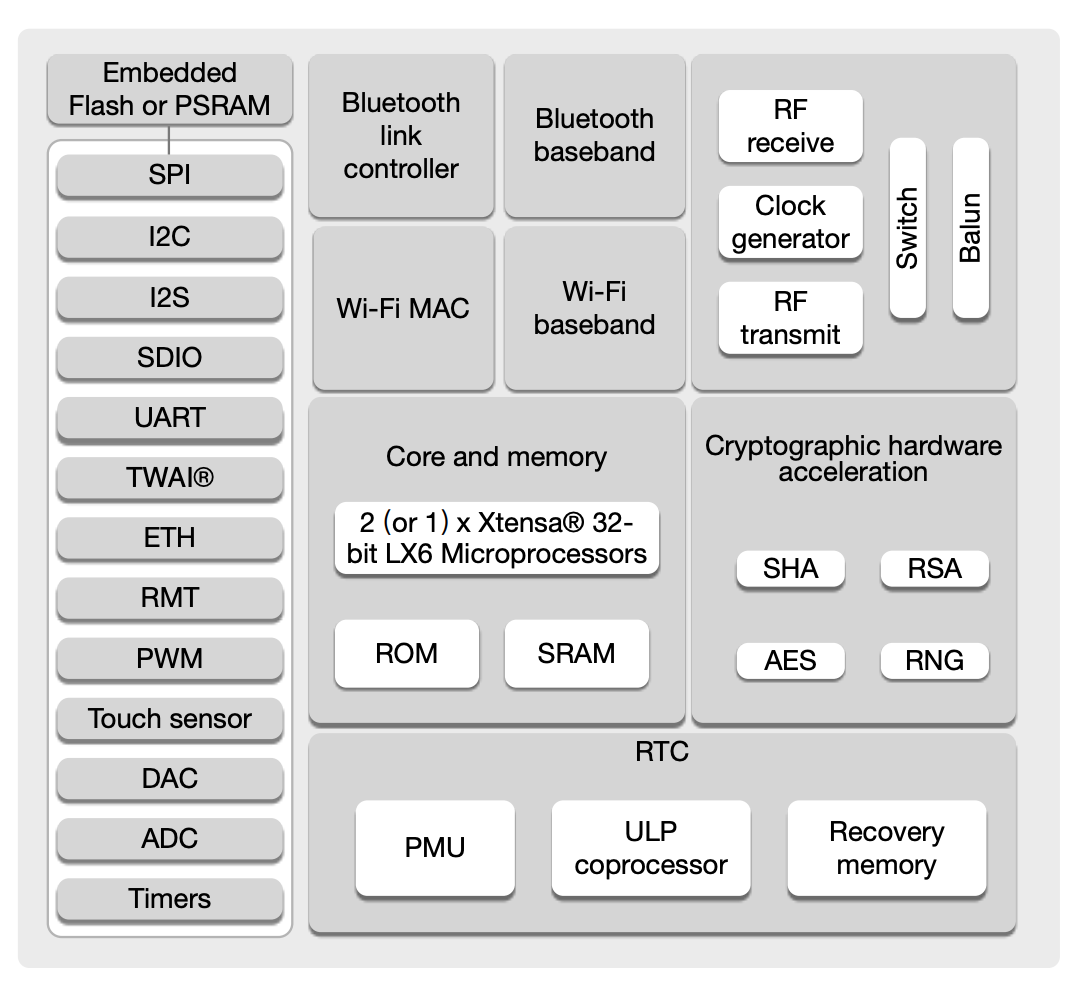
\includegraphics[width=.6\textwidth]{./Figures/esp32hardware.png}
\caption{Diagrama de bloques ESP32.}
\label{fig:diagBloques}
\end{figure}

A su vez, en la familia de ESP32 tenemos diferentes tipos de módulos [12]. Cada uno presenta pequeñas variaciones de hardware, comandos de integración de Firmware y cantidad de pines. En particular, para este trabajo se utiliza el módulo de WROOM. Más específicamente uno de los tableros de ESP32-devkit [13]. Además, existen diferentes versiones de tableros de desarrollo de WROOM para ESP32-DEVKIT. Por ello, para realizar las conexiones con los sensores, es fundamental tener conocimiento sobre la usabilidad de cada uno de los pines de la placa. Aunque esta información está disponible en la hoja de datos oficial, en caso de no tener tanto conocimiento técnico se sugiere revisar le posteo de <<ESP32 Peripherals>> en la web de RandomNerdTutorials [14], ya que es muy útil principiantes en la materia. En la figura 2.2 se presenta un diagrama de pines de dicha web.

\begin{figure}[htpb]
\centering 
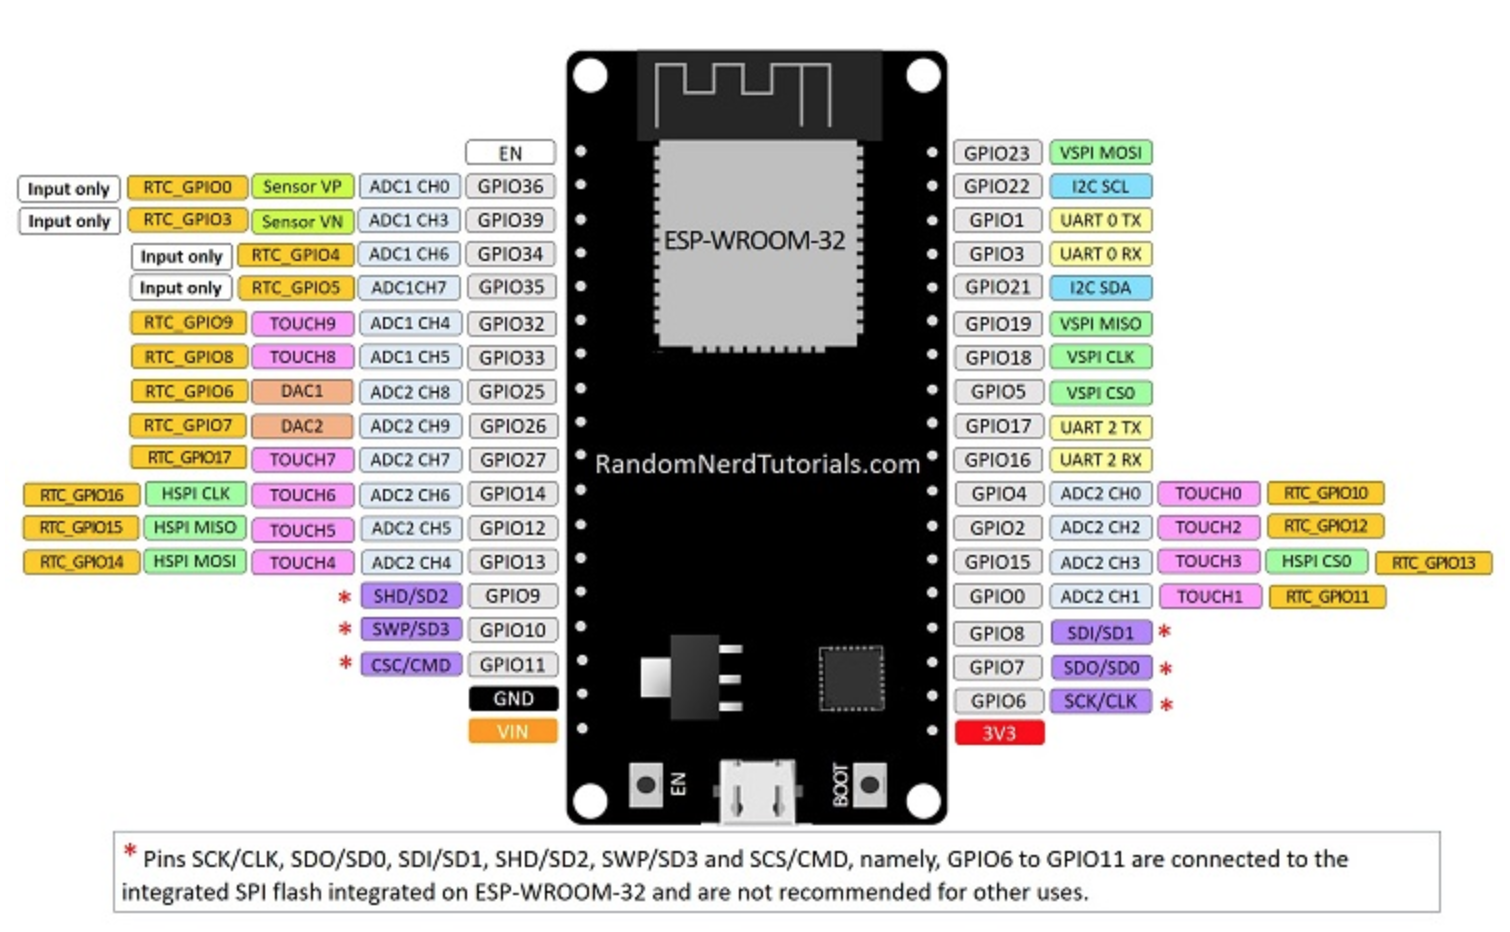
\includegraphics[width=.9\textwidth]{./Figures/esp32pines.png}
\caption{Diagrama pines ESP32.}
\label{fig:diagBloques}
\end{figure}

Para finalizar, se seleccionó esta placa no solo por lo expuesto anteriormente sobre sus bondades en hardware, sino que también, por las que tiene en software. Esto se debe a Espressif ofrece una buena variedad de ejemplos de código C en su repositorio de github [15].

\subsection{Sensor de temperatura y humedad relativa DHT11}
Con este sensor se podrá realizar la obtención de valores de temperatura y humedad ambiente. Según se detalla en su hoja de datos [16] ofrece una señal digital confiable y estable.
Este sensor cuenta con 4 pines, de los cuales usaremos los siguientes 3 (los pines se cuenta de izquierda a derecha con el sensor de frente):
\begin{itemize}
\item Pin 1: VDD (alimentación). Deberá recibir de 3,3 a 6 V. Se recomienda colocar un capacitor de 100nF entre este pin y el pin GND para su protección.
\item Pin 2: DATA. Una vez establecida la conexión, este pin enviará los datos de temperatura y humedad relativa al módulo ESP.
\item Pint 4: GND.
\end{itemize}

\subsection{Sensor de humedad en suelo capacitivo analógico V1.2}
Es un sensor se utiliza para medir la humedad del sustrato. Como se menciona en su hoja de datos [17] es una excelente opción ya que <<está hecho de un material resistente a la corrosión lo que le da una excelente vida útil>>. Cuenta con un conector de pines con las opciones de muy claros, VCC, GND y AOUT (datos analógicos). Se recomienda utilizar con una potencia entre 3,3 a 5 V.

\subsection{ADC ADS1115}
Debido a que el sensor de humedad de suelo tiene mayores pruebas usando arduido (incluso en su hoja de datos) se va a utilizar un convertidor analógico digital con el ESP32. Se utilizaron como fuentes de información su hoja de datos [18] y un tutorial de <<Programar Fácil>>[19] donde se explica su utilidad y usos. De esta forma usaremos la señal analógica del sensor capacitivo para enviar los datos digitales a la placa ESP32.

%----------------------------------------------------------------------------------------

\section{Herramientas de software}

%----------------------------------------------------------------------------------------

\section{Desarrollo UNLa}

%----------------------------------------------------------------------------------------
 
\chapter{Diseño e implementación} % Main chapter title

\section{Arquitectura del sistema}

%----------------------------------------------------------------------------------------

\section{Modelo de datos}

%----------------------------------------------------------------------------------------

\section{Modelado y confección del dispositivo }

%----------------------------------------------------------------------------------------

\section{Desarrollo del backend}

%----------------------------------------------------------------------------------------

\section{Desarrollo del frontend}

%----------------------------------------------------------------------------------------

\section{Despliegue del sistema}

%----------------------------------------------------------------------------------------

\section{Integración del sistema completo}

%----------------------------------------------------------------------------------------

\chapter{Ensayos y resultados} % Main chapter title

\subsection{Prueba de concepto del dispositivo}
En conjunto con Damian Reboredo se realizaron pruebas sobre la placa ESP32. Se logró llegar a un prototipo funcional donde los sensores descriptos anteriormente envían los datos a la placa. Además, se hizo una prueba de concepto para la apertura de la válvula. Finalmente, se realizó la programación para transmitir los datos a un servidor web, si bien los valores son fijos, se quería probar la conexión usando el protocolo HTTP. El código del proyecto se alojó en un repositorio de la organización de proyectos del laboratorio [25].

%----------------------------------------------------------------------------------------

\section{Banco de pruebas}

%----------------------------------------------------------------------------------------

\section{Pruebas de componentes}

%----------------------------------------------------------------------------------------

\section{Pruebas del backend}

%----------------------------------------------------------------------------------------

\section{Pruebas del frontend}

%----------------------------------------------------------------------------------------

\section{Valor agregado del proyecto}

%----------------------------------------------------------------------------------------
 
\chapter{Conclusiones} % Main chapter title

\section{Resultados obtenidos}

%----------------------------------------------------------------------------------------
\section{Trabajo futuro}


\begin{thebibliography}{X}

\bibitem{SobAl} \textsc{Patricia Agosto} y \textsc{Marielle Palau},
\textit{Hacia la construcción de la soberanía alimentaria}, Paraguay y Argentina, 2015.

\bibitem{EmpVer} \textsc{Organización de las Naciones Unidas para la Alimentación y la Agricultura}, \textit{Estudio del empleo verde, actual y potencial, en el sector de bioenergías}, Salta, Argentina, 2019.

\bibitem{Agri40} \textsc{Ajay Kumar Kaviti}, \textsc{Amit Kumar Thakur}, \textsc{Anita Gehlot} y \textsc{Rajesh Singh}, \textit{Internet of Things for Agriculture 4.0}, 2022.

\bibitem{Piw} \textsc{Universidad de Chile},
\textit{Proyecto Piwkeyewün}, URL: \textit{https://pueblosindigenas.ing.uchile.cl/proyecto-piwkeyewun/}, Link 2023.

\bibitem{P1} \textsc{Cortes-Cadavid Valeria} y \textsc{Vargas-García, Marco Fabian},
\textit{Diseño e implementación de un sistema de riego automatizado y monitoreo de variables ambientales mediante Iot en los cultivos urbanos de la fundación mujeres empresarias Maria Poussepin},  URL: \url{https://repositorioslatinoamericanos.uchile.cl/handle/2250/3430048}, Universidad Católica de Colombia, Colombia, Link 2023.

\bibitem{P1} \textsc{Ramírez Díaz}, \textsc{Eliécer Jesús Vergara Sierra} y \textsc{Jesús David}, \textit{Sistema de riego automatizado basado en iot utilizando variables ambientales para cultivos de berenjena en la finca la esperanza del municipio de Chinú-Córdoba},  URL: \url{https://repositorio.unicordoba.edu.co/handle/ucordoba/2706}, Universidad de Córdoba, Colombia, Link 2023.

\bibitem{P1} \textsc{Burramuño González Rocío Elena},
\textit{Sistema automatizado para riego en huertos urbanos y plantas},  URL: \url{https://repositorio.usm.cl/handle/11673/50443?show=full}, Universidad Técnica Federico Santa Maria, Chile, Link 2023.

\end{thebibliography}

%----------------------------------------------------------------------------------------
%	CONTENIDO DE LA MEMORIA  - APÉNDICES
%----------------------------------------------------------------------------------------

\appendix % indicativo para indicarle a LaTeX los siguientes "capítulos" son apéndices

% Incluir los apéndices de la memoria como archivos separadas desde la carpeta Appendices
% Descomentar las líneas a medida que se escriben los apéndices

%\include{Appendices/AppendixA}
%\include{Appendices/AppendixB}
%\include{Appendices/AppendixC}

%----------------------------------------------------------------------------------------
%	BIBLIOGRAPHY
%----------------------------------------------------------------------------------------

\Urlmuskip=0mu plus 1mu\relax
\raggedright
\printbibliography[heading=bibintoc]

%----------------------------------------------------------------------------------------

\end{document}  
